\documentclass[10pt,a4paper]{article}

% ---------- Packages ----------
\usepackage[margin=1.8cm]{geometry}   % narrow margins so everything fits on one page
\usepackage[T1]{fontenc}
\usepackage{lmodern}
\usepackage{microtype}
\usepackage{amsmath}
\usepackage{booktabs}                 % nicer tables
\usepackage{enumitem}                 % compact lists
\usepackage{tikz}                     % block diagram
\usetikzlibrary{arrows.meta,positioning,calc}
\usepackage{titlesec}
\usepackage{hyperref}

% ---------- Compact layout ----------
\pagestyle{empty}
\setlength{\parindent}{0pt}
\setlength{\parskip}{3pt}
\setlist{nosep,leftmargin=1.2em}
\titleformat{\section}{\large\bfseries}{}{0pt}{}
\titlespacing*{\section}{0pt}{7pt}{3pt}

% ---------- Block diagram styles ----------
\tikzset{
  blk/.style={draw, rectangle, rounded corners=1pt, minimum height=8mm,
              minimum width=21mm, align=center, font=\footnotesize},
  arr/.style={-{Stealth[length=1.8mm]}, thick},
  lbl/.style={font=\scriptsize}
}

\begin{document}

% ---------- Title block ----------
\begin{center}
  {\Large\bfseries Mini-Project Proposal: 6-bit, 1\,MS/s SAR ADC}\\[2pt]
  Advanced Microelectronics with Cadence --- JUNIA / IEMN \\[2pt]
  \textbf{Group members:} Member One, Member Two \hfill \textbf{Date:} \today
\end{center}

% ---------- Objective ----------
\section{1. Objective}
We will design and simulate a 6-bit successive-approximation-register (SAR) analog-to-digital
converter. Following the course flow, we first define the specifications and architecture, then build a
behavioral model and testbench, and finally replace blocks with transistor-level (analog) and
RTL/gate-level (digital) implementations for mixed-signal simulation. The SAR architecture is a good fit
because it combines a small analog core (comparator, capacitor array) with a digital control FSM, which
exercises both halves of the course.

% ---------- Specs ----------
\section{2. Target Specifications}
\begin{center}
\small
\begin{tabular}{@{}lll@{\hspace{1.2cm}}lll@{}}
\toprule
\textbf{Parameter} & \textbf{Value} & & \textbf{Parameter} & \textbf{Value} \\
\midrule
Resolution        & 6 bits             & & Sampling rate & 1\,MS/s ($T_s = 1\,\mu$s) \\
Reference voltage & $V_{ref} = 1$\,V   & & Input range   & 0--1\,V (single-ended) \\
LSB size          & $V_{ref}/2^6 = 15.6$\,mV & & Ideal SQNR & $6.02N+1.76 \approx 37.9$\,dB \\
\bottomrule
\end{tabular}
\end{center}

% ---------- Architecture ----------
\section{3. Proposed Architecture}
The input is sampled onto a binary-weighted capacitive DAC (CDAC). On each clock cycle a StrongARM
comparator compares the CDAC output with the reference level and the SAR logic keeps or drops the bit under
test, performing a binary search from MSB to LSB. With 1 sampling cycle plus 6 comparison cycles, we plan an
internal bit clock of about 8\,MHz (125\,ns period), giving some margin for settling within the 1\,$\mu$s
conversion period.

\begin{center}
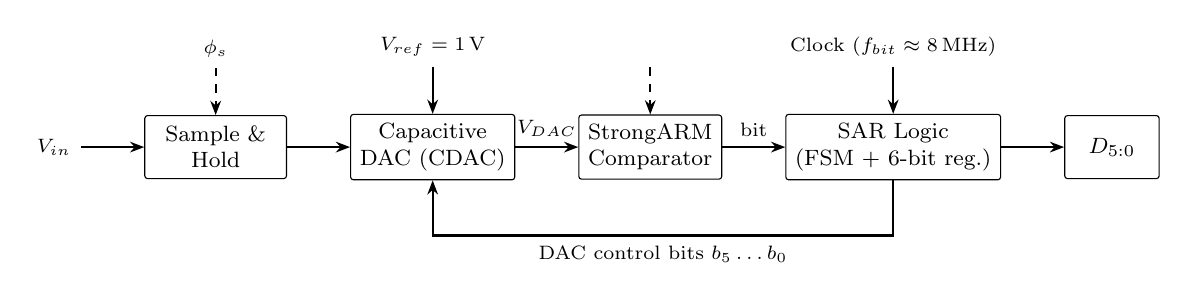
\begin{tikzpicture}[node distance=8mm]
  \node[blk, minimum width=18mm] (sh)  {Sample \&\\Hold};
  \node[blk, right=of sh,  minimum width=18mm] (dac) {Capacitive\\DAC (CDAC)};
  \node[blk, right=of dac, minimum width=18mm] (cmp) {StrongARM\\Comparator};
  \node[blk, right=of cmp, minimum width=22mm] (sar) {SAR Logic\\(FSM + 6-bit reg.)};
  \node[blk, right=of sar, minimum width=12mm] (out) {$D_{5:0}$};

  \draw[arr] ($(sh.west)+(-8mm,0)$) node[left,lbl]{$V_{in}$} -- (sh);
  \draw[arr] (sh) -- (dac);
  \draw[arr] (dac) -- node[above,lbl]{$V_{DAC}$} (cmp);
  \draw[arr] (cmp) -- node[above,lbl]{bit} (sar);
  \draw[arr] (sar) -- (out);
  \draw[arr] (sar.south) -- ++(0,-7mm) -| node[below,lbl,pos=0.25]{DAC control bits $b_5\ldots b_0$} (dac.south);
  \draw[arr] ($(dac.north)+(0,6mm)$) node[above,lbl]{$V_{ref}=1$\,V} -- (dac.north);
  \draw[arr] ($(sar.north)+(0,6mm)$) node[above,lbl]{Clock ($f_{bit}\approx 8$\,MHz)} -- (sar.north);
  \draw[arr, dashed] ($(cmp.north)+(0,6mm)$) -- (cmp.north);
  \draw[arr, dashed] ($(sh.north)+(0,6mm)$) node[above,lbl]{$\phi_s$} -- (sh.north);
\end{tikzpicture}
\end{center}

\vspace{-2pt}
\textbf{Blocks:}
\begin{itemize}
  \item \textbf{CDAC:} binary-weighted array ($32C, 16C, 8C, 4C, 2C, C$ plus a dummy $C$, 64\,$C_u$ total);
        unit capacitor sized for matching and $kT/C$ noise well below $\tfrac12$\,LSB.
  \item \textbf{Comparator:} StrongARM latch (dynamic, clocked, low static power), with input-referred offset below $\tfrac12$\,LSB.
  \item \textbf{Sample \& Hold:} MOS switch sampling $V_{in}$ onto the CDAC top plate (charge injection and
        settling to be checked).
  \item \textbf{SAR logic:} synchronous FSM written in HDL (SystemVerilog/Verilog), synthesized to gates.
  \item \textbf{Clock:} external ideal source, with non-overlapping phases for sample and convert.
\end{itemize}

% ---------- Plan ----------
\section{4. Work Plan and Deliverables}
\begin{enumerate}
  \item \textbf{Specifications and architecture} (this proposal).
  \item \textbf{Behavioral model} of the full ADC (Verilog-A / Verilog-AMS) and testbench: ramp and sine inputs.
  \item \textbf{Block-level design and simulation} (at least one block, as required): StrongARM comparator and CDAC
        in Virtuoso (transient, offset, and speed); SAR FSM in RTL with Xcelium simulation.
  \item \textbf{Mixed-signal integration:} replace behavioral blocks with the transistor-level and gate-level netlists.
  \item \textbf{Performance extraction} (optional): offset, gain error, DNL, INL, SNR/ENOB from a coherent-sine or ramp test.
  \item \textbf{Final presentation} (W46) and report.
\end{enumerate}

\textbf{Success criteria:} correct 6-bit output codes across 0--1\,V at 1\,MS/s, with $|\mathrm{DNL}|,|\mathrm{INL}| < 1$\,LSB in
simulation.

\end{document}
